%----------------------------------------------------------------------
% Harnessing cloud computing for high capacity analysis of neuroimaging
% data from NDAR
%
% Poster for OHBM 2015
%
% Contributing authors: Daniel Clark, Cameron Craddock
%----------------------------------------------------------------------

%----------------------------------------------------------------------
% Document class, packages, and formatting
%----------------------------------------------------------------------
\documentclass[final,hyperref={pdfpagelabels=false}]{beamer}

%% Packages
\usepackage{grffile}
\usepackage[english]{babel}
\usepackage[latin1]{inputenc}
\usepackage{amsmath,amsthm, amssymb, latexsym}
%\usepackage[framemethod=tikz]{mdframed}
%\usepackage{times}\usefonttheme{professionalfonts}  % obsolete
%\usefonttheme[onlymath]{serif}
%\boldmath
\usepackage{graphicx}
\usepackage{enumerate}
%\usepackage[orientation=portrait,size=custom,width=83.96,height=101,scale=1]{beamerposter}
\usepackage[orientation=portrait,size=custom,width=141,height=140,scale=1]{beamerposter}
%\usepackage[orientation=portrait,width=89,height=102,scale=1.1,debug]{beamerposter}
%\usepackage[orientation=portrait,size=a0,scale=1.4,debug]{beamerposter}
% change list indention level
% \setdefaultleftmargin{3em}{}{}{}{}{}
%\usepackage{snapshot} % will write a .dep file with all dependencies, allows for easy bundling

\usepackage{array,booktabs,tabularx}

%% Formatting
\mode<presentation>{\usetheme{CMINKI}}
\newcolumntype{Z}{>{\centering\arraybackslash}X} % centered tabularx columns
\newcommand{\pphantom}{\textcolor{ta3aluminium}} % phantom introduces a vertical space in p formatted table columns??!!
% Column sizing
\newlength{\columnheight}
\setlength{\columnheight}{72cm}

%\graphicspath{{figures/}}
\listfiles

%----------------------------------------------------------------------
% Title Block
%----------------------------------------------------------------------
%% Title
\title{\vskip1ex\Huge Harnessing cloud computing for high capacity analysis of neuroimaging data from NDAR}

%% Author
\author{\Large Daniel Clark$^1$, Christian Haselgrove$^2$, David Kennedy$^2$, Zhizhong Liu$^3$,\\[.5ex]Michael Milham$^1$, Petros Petrosyan$^4$, Carinna Torgerson$^3$, John Van Horn$^3$, Cameron Craddock$^1$}
\institute[NKI]{$^1$Child Mind Institute, New York, NY, $^2$ University of Massachuttes Medical School, Worcester, MA, $^3$University of Southern California, Los Angeles, CA, $^4$UCLA, Los Angeles, CA, $^5$Nathan S. Kline Institute for Psychiatric Research, Orangeburg, NY}

%% Poster info
\posternum{\Large 3535 Thursday 12:45}
\date[June 18th, 2015]{June 18th, 2015}

%----------------------------------------------------------------------
% Poster content
%----------------------------------------------------------------------
\begin{document}
\begin{frame}
    \begin{columns}
    %----------------------------------------------------------------------
    % Right column of poster
    %----------------------------------------------------------------------
    % Set up a column
    \begin{column}{.5\textwidth}
    %\begin{beamercolorbox}[center,wd=\textwidth]{postercolumn}
    %\begin{minipage}[T]{.98\textwidth}  % tweaks the width, makes a new \textwidth
        \parbox[t][\columnheight]{\textwidth}{ % must be some better way to set the the height, width and textwidth simultaneously
        %----------------------------------------------------------------------
        % Introduction
        %----------------------------------------------------------------------
        \begin{block}{Introduction}
            \begin{itemize}
                \item The National Database for Autism Research (NDAR)$^{1}$ hosts a vast collection of neuroimaging datasets that can be processed and utilized to yield significant scientific discoveries.
                \item This amount of resources necessitates a high-performance computing (HPC) infrastructure, which is not always readily available for researchers in-house.
                \item Amazon Web Services (AWS) Elastic Compute Cloud (EC2) computing service offers a ``pay as you go" model that allows researchers to utilize HPC performance without the up-front captial costs and maintenance of an in-house solution.
                \item The developers of the Laboratory of Neuro Imaging (LONI) Pipeline, the Neuroimaging Informatics Tools and Resources Clearinghouse (NITRC) Computational Environment (CE) and the Configurable Pipeline for the Analysis of Connectomes (C-PAC) have implemented pipelines in EC2 that interface with NDAR
                \item The developers of the Laboratory of Neuro Imaging (LONI) Pipeline, the Neuroimaging Informatics Tools and Resources Clearinghouse (NITRC) Computational Environment (CE) and the
            \end{itemize}
        \vfill
        \end{block}
        %----------------------------------------------------------------------
        % Methods
        %----------------------------------------------------------------------
        \begin{block}{Methods}
            \vskip1ex
            %% LONI pipeline
            \begin{column}{.5\textwidth}
                {\bf LONI Pipeline}
                \begin{itemize}
                    \item The LONI Pipeline software was extended to include new pipeline modules to access data from the NDAR database, transfer input data out of Amazon S3 (Simple Storage Service), and to load results back into S3$^{2}$
                    \item A pipeline was constructed to extract cortical thickness and subcortical region volume data from structural MRI images in the NDAR database, which included:
                    \begin{enumerate}
                        \item Reorient images to standard orientation using FSL's reorient2std module
                        \item Extract cortical thickness using FreeSurfer recon-all
                        \item Calculate volumes of subcortical regions using FSL's BET and FIRST all
                    \end{enumerate}
                    \item The resulting pipeline was used to process 780 T1-weighted structural images and return the results to NDAR
                \end{itemize}
                \vskip1ex
                {\bf Configurable Pipeline For the Analysis of Connectomes (C-PAC)$^{3}$}
                \begin{itemize}
                    \item C-PAC modules were written in Python to build input data lists by querying NDAR, read input data from S3, write processed results to S3 and write values back to the NDAR database
                    \item New pipelines were created to perform the ANTS cortical thickness$^{4}$ procedure and the Preprocessed Connectomes Project's Quality Assessment Protocol (\url{http://preprocessed-connectomes-project.github.io/quality-assessment-pipeline})$^{5}$
                    \item The resulting pipelines and modules were used to process several datasets and return the results to NDAR
                        \begin{enumerate}
                            \item Cortical extraction from 3,197 T1-weighted structural images
                            \item Structural and functional processing for 1,112 datasets from ABIDE
                            \item Automated quality asssessment of 1,112 datasets from ABIDE
                        \end{enumerate}
                \end{itemize}
				\vskip3ex
                %% NITRC-CE pipeline
                {\bf Neuroimaging Informatics Tools and Resources Clearinghouse Computational Environment (NITRC-CE)$^{6}$}
                \begin{itemize}
                    \item The NITRC pipeline processed data using three primary utilities
                        \begin{enumerate}
                            \item Extract anatomical and surface-base measures with Freesurfer recon-all
                            \item Segment subcortical structures using FSL's FIRST to produce volumetric and mesh outputs
                            \item Time series QA measures using the fmriqa\_generate.pl utility from the BXH/XCEDE Tools suite, including mean intensty, center of mass, per-slice variation, and others
                        \end{enumerate}
                    \item Python modules were created to query and download data from NDAR as well as to store results back to their database
                    \item The recon-all and FIRST tools processed 986 and 1,247 T1-weighted anatomical scans, respectively; the fmriqa\_generate QA measures were generated from 1,349 functional scans.
                \end{itemize}
				\vskip3ex
	            {\bf Interacting with the NDAR database}
	                \begin{itemize}
	                    \item Launched an AWS-hosted miNDAR database by querying NDAR website for the data of interest (e.g. from a particular study)
	                    \item Built a subject list by querying the database for subjects of interest to pass to our pipeline
	                    \item Launch an AWS EC2 HPC cluster using Starcluster$^{7}$
	                    \item Log into the cluster and submit a Sun Grid Engine job using our pipeline software and the subject list
	                    \item The pipeline software will process the data, store raw outputs in an AWS S3 bucket and insert S3 filepaths and output measures into miNDAR database
	                \end{itemize}
					\vskip3ex
	              %% EC2 Spot pricing
	              {\bf EC2 Spot Pricing}
	              \begin{itemize}
	                  \item In addition to the ``pay as you go" compute pricing model, AWS offers users to bid on instances that are not being used
	                  \item As opposed to paying an ``on-demand" fixed price, the hourly charge for the instances will vary over time based on what people in different regions are willing to pay
	                  \item If the spot market price goes above what the user bids, their instance will be terminated by Amazon and all of their processes will be stopped and their data lost
	                  \item Typically, one can expect to pay one-eighth of the hourly price of a standard on-demand instance when using spot-pricing
	                  \item AWS offers cloud solutions based on geographic region, where the price for services vary
	                  \item Some regions fluxuate on spot price more than others, but there are ways to minimize process interruptions and lost data in how one configures their cluster and pipelines
	              \end{itemize}
				
            \end{column}
            \begin{column}{.5\textwidth}
                %% LONI pipeline figure
                \begin{figure}
                    \begin{center}
                        \includegraphics[width=.9\textwidth]{loni_pipeline.eps}
                    \end{center}
                    \caption{\label{fig:loni_pipe}Graphical layout of the constructed pipeline}
                \end{figure}
                \vskip3ex			
                  \begin{figure}
                      \begin{center}
                          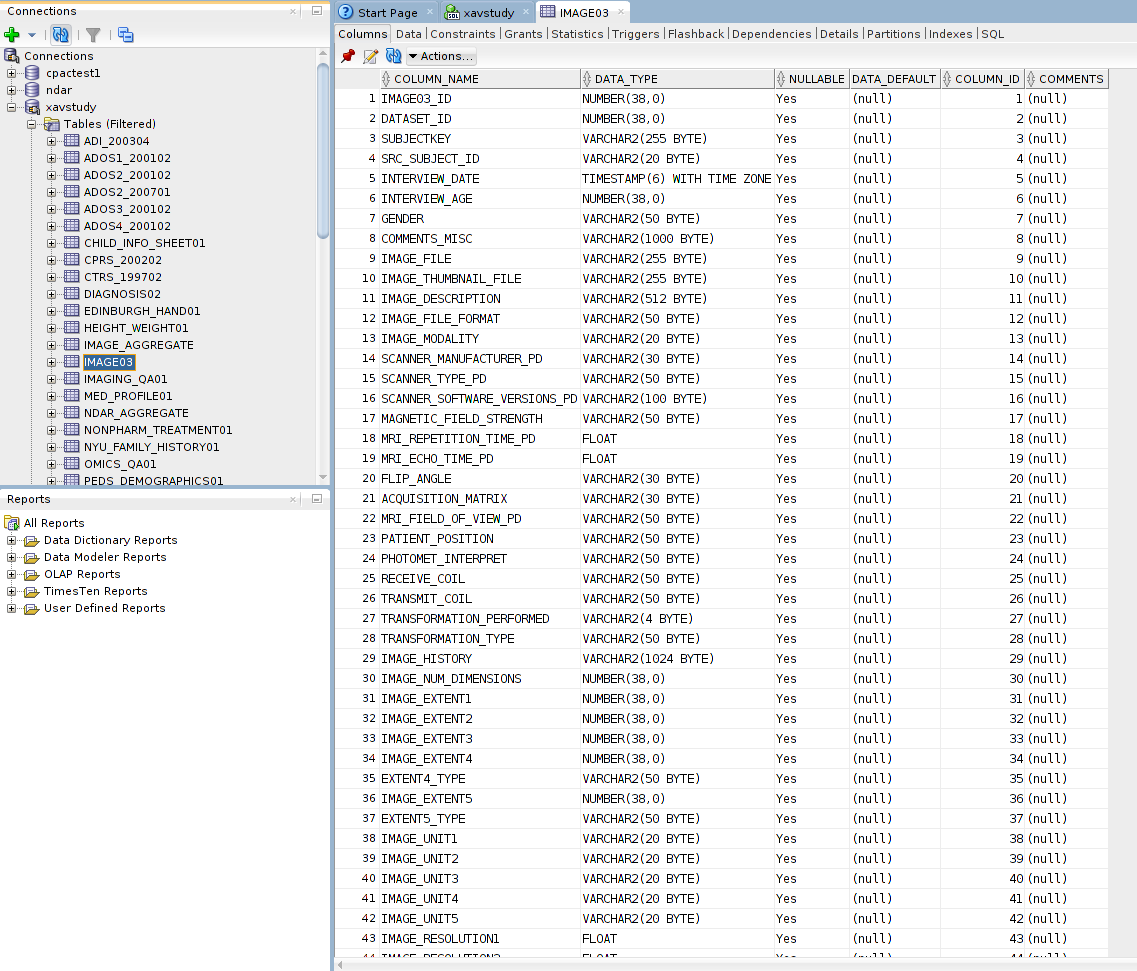
\includegraphics[width=.9\textwidth]{mindar.png}
                      \end{center}
                      \caption{\label{fig:mindar}miNDAR database}
                  \end{figure}
              \vskip3ex
                %% Spot history figure
                \begin{figure}
                    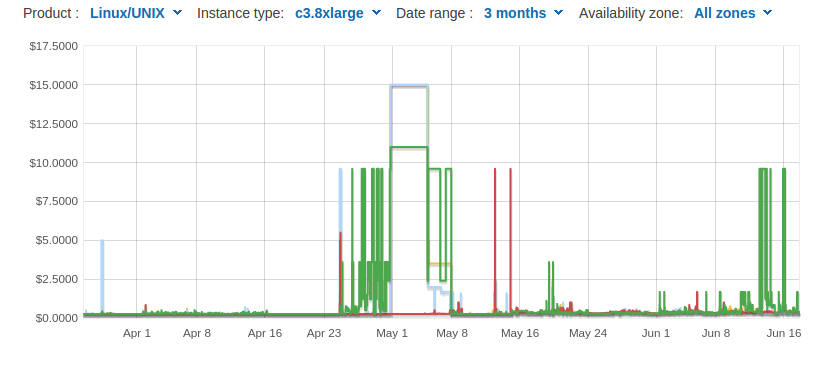
\includegraphics[width=.99\textwidth]{spot_history.png}
                    \caption{\label{fig:spot_history}Spot price history for the c3.8xlarge instance in the us-east-1 region on AWS across the four different availability zones for the past three months}
                \end{figure}
					
				
            \end{column}
        \vfill
        \end{block}
        \begin{block}{Results}
            \begin{center}
                %% Preprocessing results table
                \begin{table}
                    \caption{Processing completed as a part of the effort. Nodes corresponds to the number of hosts used in the calculation. PF is parallelization factor and corresponds to the number of jobs ran in parallel on each node. On demand instances were used for the master node and spot instances were used for all computation nodes in the cluster. CPU Time is the total amount of time required to perform the computation and Wall Time is the amount of time that passed. \# DS: Number of datasets. CPD: Cost Per Dataset. C-PAC: Configurable Pipeline for the Analysis of Connectomes. NITRC-CE: NITRC Computational Environment}
                    \vskip2ex
                    \begin{tabularx}{\textwidth}{XXlrl*{6}{r}}
                        {\bf Processing} & {\bf \# DS} & {\bf Platform} & {\bf Nodes} & {\bf PF} & {\bf CPU Time} & {\bf Wall Time} & {\bf Cost} & {\bf CPD}\\
                        \hline
                        ANTS Cortical Thickness & 3197 &  & 20 & 8 & 23,018 & 147 & \$760.24 & \$0.24\\
                        Resting state fMRI processing w/ 4 strategies & 1112 & C-PAC  & 20 & 3 & 834 & 22 & \$80.54 & \$0.07\\
                        Quality Assessment Protocol & 1112 & & 20 & 4 & 380 & 14 & \$19.02 & \$0.02\\
                        \hline
                        Freesurfer recon-all & 986 &  & 4 & 32 & 23,664 & 193 & \$211.44 & \$0.21\\
                        FSL FIRST & 1247 & NITRC-CE & 4 & 32 & 208 & 3 & \$2.19 & $>$ \$0.01\\
                        Temporal QA & 1349 &  & 4 & 32 & 450 & 13 & \$4.69 & $>$ \$0.01\\
                        \hline
                        Freesurfer recon-all and FSL FIRST & 780 & LONI Pipeline & 20 & 32 & 18,720 & 49 & \$252.36 & \$0.32\\
                    \end{tabularx}
                \end{table}
            \end{center}
			\vskip2ex
            {\bf Benefits of the cloud}
            \begin{itemize}
                \item The scalability and payment model for processing this data on a cloud platform allowed for an efficient processing of the NDAR datasets, both in time and cost
                \item Additionally, there was no need to install, configure, and maintain machines locally, saving on overhead
                \item Competition for computing resources was controlled as every cluster launch was done by the user doing the processing; no fellow researchers needed to login and use additional computing power
                \item Cost and time models were produced to demonstrate the benefits of using cloud computing for increasingly large datasets
            \end{itemize}
	        \vfill
	        \end{block}
			
          }
        %\end{minipage}
      %\end{beamercolorbox}
    \end{column}
    %----------------------------------------------------------------------
    % Right column of poster
    %----------------------------------------------------------------------
    % Set up a column
    \begin{column}{.5\textwidth}
    %\begin{beamercolorbox}[center,wd=\textwidth]{postercolumn}
    %\begin{minipage}[T]{.98\textwidth} % tweaks the width, makes a new \textwidth
        \parbox[t][\columnheight]{\textwidth}{ % must be some better way to set the the height, width and textwidth simultaneously
        %----------------------------------------------------------------------
        % Results
        %----------------------------------------------------------------------
        \begin{block}{Results cont.}
            %\vskip4ex
            %% Costs and run time models
            {\bf Costs and run time models}
            \begin{itemize}
                \item Models assume user uploads their input data to the cloud, runs their pipelines and (optionally) downloads their outputs as they become available.
                \item Outputs are stored on an AWS Elastic Block Store (EBS) hard drive mounted to the master node and is NFS-shared across all of the slave nodes.
                \item Users can also upload their processed outputs to a cloud storage solution, like AWS Simple Storage Service (S3) directly from the cluster - this is the approach that was taken in processing data for NDAR.
                \item Storing results in AWS S3 avoids costly download time and provides for a viable solution for backing up data; however this does incur additional storage costs.
            \end{itemize}
		 \vskip3ex
          %% Left column
          \begin{column}{.47\textwidth}
              \begin{figure}
                  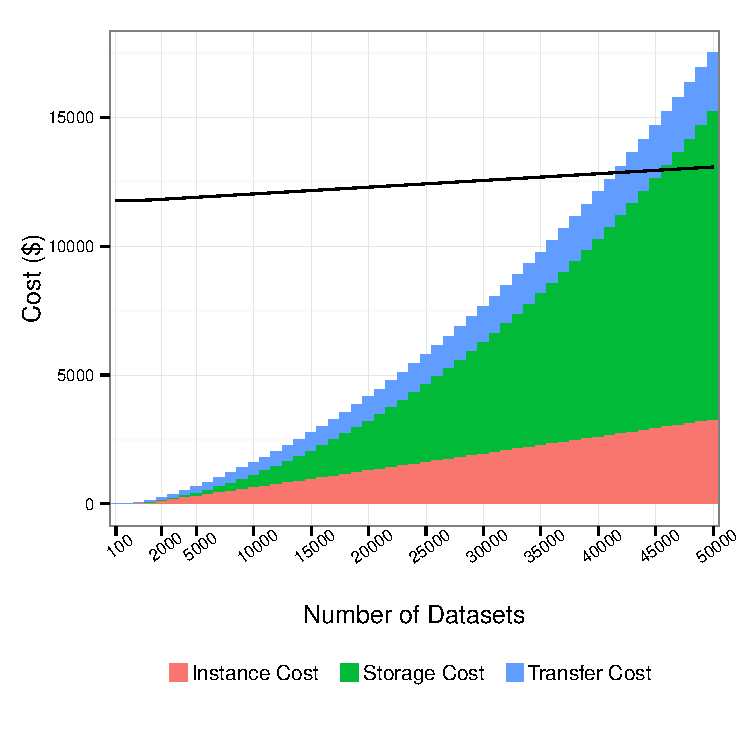
\includegraphics[width=.99\textwidth]{cpac-costs.pdf}
                  \caption{\label{fig:cpac-costs}AWS EC2 costs, grouped by cost type, for a typical C-PAC pipeline for different sized datasets versus owning and maintaining own server; costs are based on using the cluster configuration shown in Table 1 for the cloud, and a single compute node locally}
              \end{figure}
              %% Freesurfer costs figure
              \begin{figure}
                  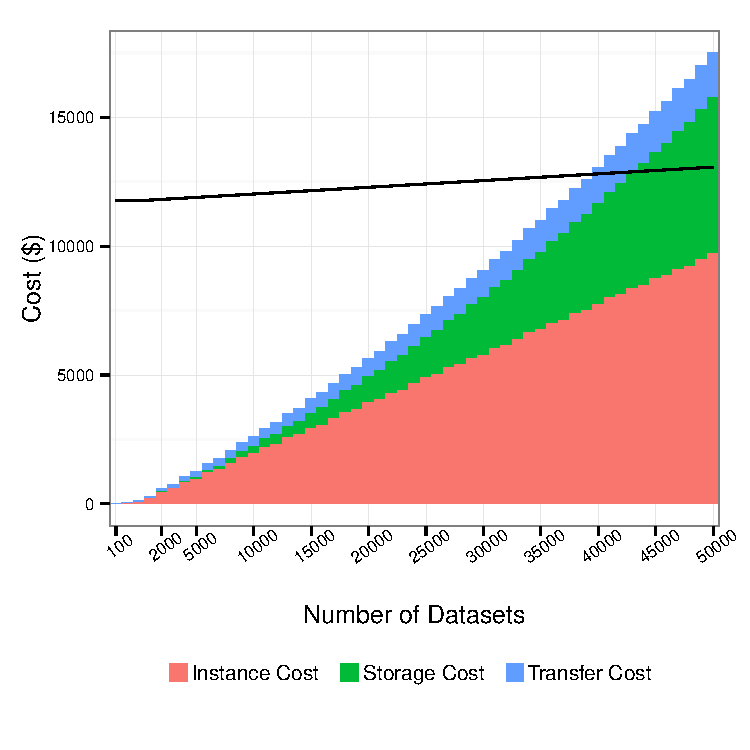
\includegraphics[width=.99\textwidth]{fs-costs.pdf}
                  \caption{\label{fig:fs-costs}AWS EC2 costs, grouped by cost type, for a typical Freesurfer pipeline for different sized datasets versus owning and maintaining own server; costs are based on using the cluster configuration shown in Table 1 for the cloud, and a single compute node locally}
              \end{figure}
              \end{column}
          %% Right column
          \begin{column}{.47\textwidth}

              %% C-PAC times figure
              \begin{figure}
                  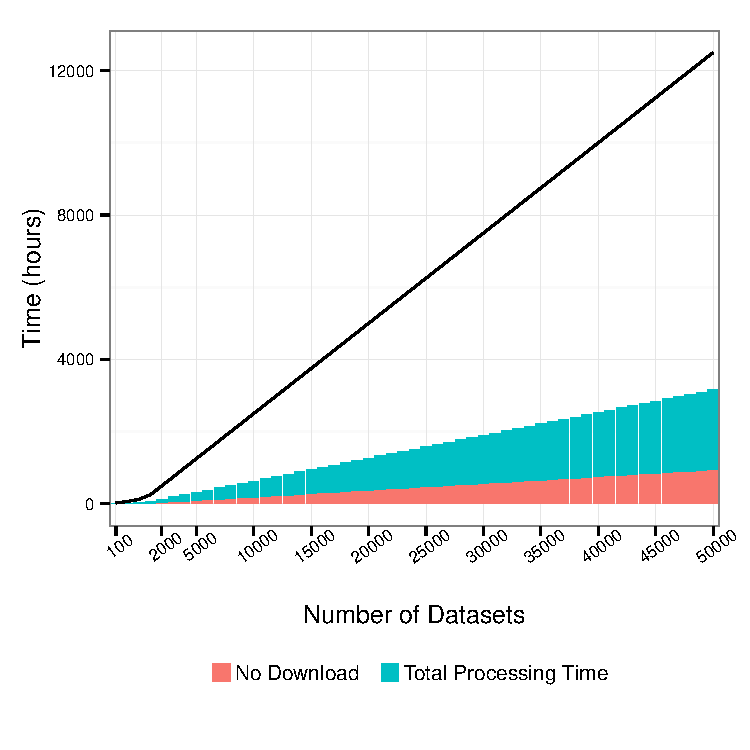
\includegraphics[width=.99\textwidth]{cpac-times.pdf}
                  \caption{\label{fig:cpac-times}Run times using the C-PAC pipeline, grouped by downloading vs non-downoading output data, for different sized datasets versus running locally; times are based on using the cluster configuration shown in Table 1 for the cloud, and a single compute node locally}
              \end{figure}
              %% Freesurfer times figure
              \begin{figure}
                  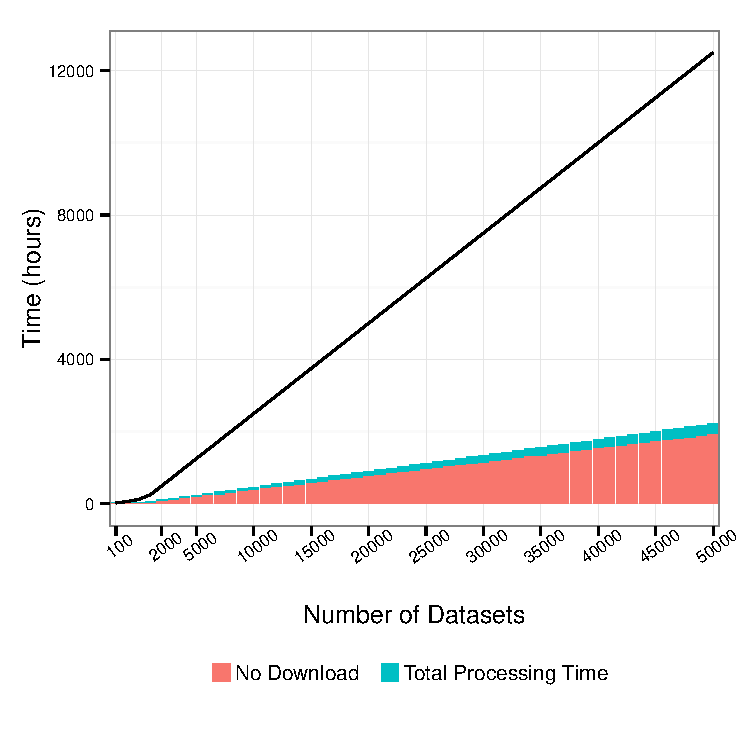
\includegraphics[width=.99\textwidth]{fs-times.pdf}
                  \caption{\label{fig:fs-times}Run times using the Freesurfer pipeline, grouped by downloading vs non-downoading output data, for different sized datasets versus running locally}
              \end{figure}
              %\begin{itemize}
              %     \item As shown in figure \ref{fig:best_worst} models learned for the best and worst performing participants match
              %           with the canonical pattern of the default network.
              %     \item The best participant was able to follow the instructures very well \ref{fig:best_worst}, the worst seems
              %           to have been corrupted by noise.
              %     \item Figure \ref{fig:inter_subject} shows 12 of the subjects were able to modulate the DN at above chance levels,
              %           performance on feedback runs is consistent independent of order, but performance on nonfeedback runs improves
              %           if they occur after feedback runs.
              %     \item Measures that were significantly associated with DN regulation include ($p<0.05$, FDR corrected):  the affect intensity measure (AIM), ruminative responses scale (RRS), and the imaginal processes inventory. 
              %\end{itemize}
          \end{column}
        \end{block}
        %----------------------------------------------------------------------
        % Conclusion
        %----------------------------------------------------------------------
        \begin{block}{Conclusion}
            \begin{itemize}
                \item NDAR provides a wealth of heterogenous data for studying the effects of autism and an excellent framework for the querying and storing of processed data
                \item Cloud computing services like AWS EC2 are viable solutions for the processing and analysis of large amounts of data
                \item A time and cost analysis argues for the benefits of using cloud computing over buying and maintaining one's own computing resource
            \end{itemize}
        \end{block}
        %----------------------------------------------------------------------
        % References and acknowledgements
        %----------------------------------------------------------------------
        \begin{block}{References and Acknowledgements}
            1. Hall, D. et al. (2012), Neuroinformatics. 10(4):331-9\\
            2. Torgerson, C.M. et al. (2015), Brain Imaging and Behavior 9:89-103\\
            3. C-PAC ref\\
            4. Das, S.R. et al. (2009), Neuroimage, 45(3): 867-79\\
            5. QAP ref\\
            6. Haselgrove, C. et al. (2014), Front. Neuroinform. 8:52\\
            7. Starcluster ref
            %9. LaConte, S.M. et al. (2011). NeuroImage, 56(2), 440-454.\\
            %10. Cox, R.W. (1996) Comput. Biomed. Res. 29: 162-173.\\
            \vskip1ex
            %% Support
            Data collection and salary support was provided by a NARSAD Young Investigator Award to RCC.
         \end{block}
          }
          % ---------------------------------------------------------%
          % end the column
      %  \end{minipage}
      %\end{beamercolorbox}
    \end{column}
    % ---------------------------------------------------------%
    % end the column
  \end{columns}
\end{frame}
\end{document}

%%%%%%%%%%%%%%%%%%%%%%%%%%%%%%%%%%%%%%%%%%%%%%%%%%%%%%%%%%%%%%%%%%%%%%%%%%%%%%%%%%%%%%%%%%%%%%%%%%%%
%%% Local Variables: 
%%% mode: latex
%%% TeX-PDF-mode: t
%%% End:
